% The taxonomy of the benchmark study: task types (the domains, level r = 2)
% nested in benchmarks (level r = 1). Two of the five benchmarks are expanded,
% and BBH shows three of its 23 task types.
% Population as in code/mixedbench/load.R: 34 task types in 5 benchmarks;
% BBH holds 23 of them, MATH 4 (four advanced subjects merged).
% Compile here: pdflatex taxonomy_tree.tex -> taxonomy_tree.pdf.
\documentclass[border=4pt]{standalone}
\usepackage{amsmath, amssymb}
\usepackage{tikz}
\usetikzlibrary{positioning, calc}
\definecolor{skyline}{RGB}{33,122,147}

\tikzset{
  every node/.style={font=\sffamily\footnotesize, text=skyline},
  lvl1/.style={draw=skyline, rounded corners=4pt, minimum width=16mm, minimum height=7.5mm, line width=0.8pt, font=\sffamily\small},
  lvl2/.style={draw=skyline, minimum height=8.5mm, line width=0.8pt, align=center, inner xsep=1.2mm, inner ysep=1mm},
  more/.style={lvl2, draw=skyline!60, dashed, text=skyline!80},
  edge/.style={draw=skyline, line width=0.6pt},
  lvllab/.style={font=\sffamily\footnotesize, text=black!55, align=right, anchor=east},
}

\begin{document}
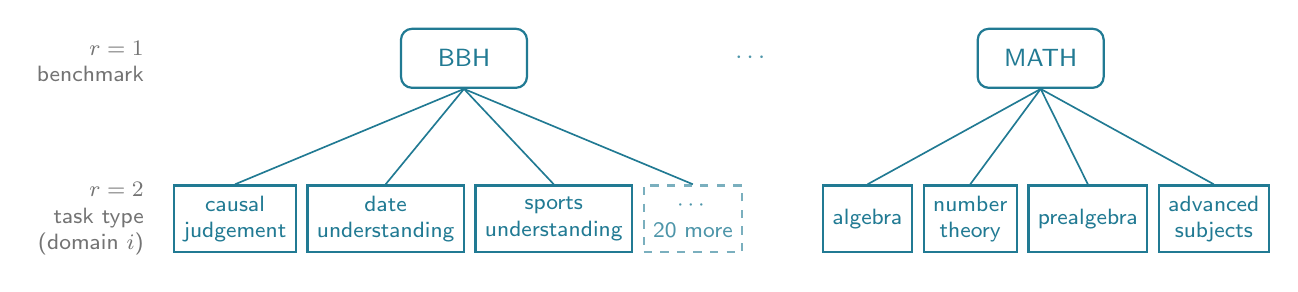
\begin{tikzpicture}[node distance=1.2mm]
  % ---- level 2: task types (the domains) ----------------------------------
  \node[lvl2] (b1) at (0,0) {causal\\judgement};
  \node[lvl2, right=of b1] (b2) {date\\understanding};
  \node[lvl2, right=of b2] (b3) {sports\\understanding};
  \node[more, right=of b3] (b4) {$\cdots$\\20 more};
  \node[lvl2, right=10mm of b4] (m1) {algebra};
  \node[lvl2, right=of m1] (m2) {number\\theory};
  \node[lvl2, right=of m2] (m3) {prealgebra};
  \node[lvl2, right=of m3] (m4) {advanced\\subjects};

  % ---- level 1: benchmarks, centred over their task types -----------------
  \node[lvl1] (bbh)  at ($(b1.north)!0.5!(b4.north) + (0,1.6)$) {BBH};
  \node[lvl1] (math) at ($(m1.north)!0.5!(m4.north) + (0,1.6)$) {MATH};
  \node[text=skyline!80, font=\sffamily\small] at ($(bbh.east)!0.5!(math.west)$) {$\cdots$};

  % ---- tree edges ----------------------------------------------------------
  \foreach \c in {b1,b2,b3,b4} \draw[edge] (bbh.south) -- (\c.north);
  \foreach \c in {m1,m2,m3,m4} \draw[edge] (math.south) -- (\c.north);

  % ---- level labels --------------------------------------------------------
  \node[lvllab] at ($(b1.west) + (-2.5mm,0) + (0,1.6) + (0,0.4)$) {$r = 1$\\benchmark};
  \node[lvllab] at ($(b1.west) + (-2.5mm,0)$) {$r = 2$\\task type\\(domain $i$)};
\end{tikzpicture}
\end{document}
